\documentclass[]{book}
\usepackage{lmodern}
\usepackage{amssymb,amsmath}
\usepackage{ifxetex,ifluatex}
\usepackage{fixltx2e} % provides \textsubscript
\ifnum 0\ifxetex 1\fi\ifluatex 1\fi=0 % if pdftex
  \usepackage[T1]{fontenc}
  \usepackage[utf8]{inputenc}
\else % if luatex or xelatex
  \ifxetex
    \usepackage{mathspec}
  \else
    \usepackage{fontspec}
  \fi
  \defaultfontfeatures{Ligatures=TeX,Scale=MatchLowercase}
\fi
% use upquote if available, for straight quotes in verbatim environments
\IfFileExists{upquote.sty}{\usepackage{upquote}}{}
% use microtype if available
\IfFileExists{microtype.sty}{%
\usepackage{microtype}
\UseMicrotypeSet[protrusion]{basicmath} % disable protrusion for tt fonts
}{}
\usepackage[margin=1in]{geometry}
\usepackage{hyperref}
\hypersetup{unicode=true,
            pdftitle={On Matters Of Nature and Science},
            pdfauthor={L A Liggett},
            pdfborder={0 0 0},
            breaklinks=true}
\urlstyle{same}  % don't use monospace font for urls
\usepackage{natbib}
\bibliographystyle{apalike}
\usepackage{color}
\usepackage{fancyvrb}
\newcommand{\VerbBar}{|}
\newcommand{\VERB}{\Verb[commandchars=\\\{\}]}
\DefineVerbatimEnvironment{Highlighting}{Verbatim}{commandchars=\\\{\}}
% Add ',fontsize=\small' for more characters per line
\usepackage{framed}
\definecolor{shadecolor}{RGB}{248,248,248}
\newenvironment{Shaded}{\begin{snugshade}}{\end{snugshade}}
\newcommand{\KeywordTok}[1]{\textcolor[rgb]{0.13,0.29,0.53}{\textbf{#1}}}
\newcommand{\DataTypeTok}[1]{\textcolor[rgb]{0.13,0.29,0.53}{#1}}
\newcommand{\DecValTok}[1]{\textcolor[rgb]{0.00,0.00,0.81}{#1}}
\newcommand{\BaseNTok}[1]{\textcolor[rgb]{0.00,0.00,0.81}{#1}}
\newcommand{\FloatTok}[1]{\textcolor[rgb]{0.00,0.00,0.81}{#1}}
\newcommand{\ConstantTok}[1]{\textcolor[rgb]{0.00,0.00,0.00}{#1}}
\newcommand{\CharTok}[1]{\textcolor[rgb]{0.31,0.60,0.02}{#1}}
\newcommand{\SpecialCharTok}[1]{\textcolor[rgb]{0.00,0.00,0.00}{#1}}
\newcommand{\StringTok}[1]{\textcolor[rgb]{0.31,0.60,0.02}{#1}}
\newcommand{\VerbatimStringTok}[1]{\textcolor[rgb]{0.31,0.60,0.02}{#1}}
\newcommand{\SpecialStringTok}[1]{\textcolor[rgb]{0.31,0.60,0.02}{#1}}
\newcommand{\ImportTok}[1]{#1}
\newcommand{\CommentTok}[1]{\textcolor[rgb]{0.56,0.35,0.01}{\textit{#1}}}
\newcommand{\DocumentationTok}[1]{\textcolor[rgb]{0.56,0.35,0.01}{\textbf{\textit{#1}}}}
\newcommand{\AnnotationTok}[1]{\textcolor[rgb]{0.56,0.35,0.01}{\textbf{\textit{#1}}}}
\newcommand{\CommentVarTok}[1]{\textcolor[rgb]{0.56,0.35,0.01}{\textbf{\textit{#1}}}}
\newcommand{\OtherTok}[1]{\textcolor[rgb]{0.56,0.35,0.01}{#1}}
\newcommand{\FunctionTok}[1]{\textcolor[rgb]{0.00,0.00,0.00}{#1}}
\newcommand{\VariableTok}[1]{\textcolor[rgb]{0.00,0.00,0.00}{#1}}
\newcommand{\ControlFlowTok}[1]{\textcolor[rgb]{0.13,0.29,0.53}{\textbf{#1}}}
\newcommand{\OperatorTok}[1]{\textcolor[rgb]{0.81,0.36,0.00}{\textbf{#1}}}
\newcommand{\BuiltInTok}[1]{#1}
\newcommand{\ExtensionTok}[1]{#1}
\newcommand{\PreprocessorTok}[1]{\textcolor[rgb]{0.56,0.35,0.01}{\textit{#1}}}
\newcommand{\AttributeTok}[1]{\textcolor[rgb]{0.77,0.63,0.00}{#1}}
\newcommand{\RegionMarkerTok}[1]{#1}
\newcommand{\InformationTok}[1]{\textcolor[rgb]{0.56,0.35,0.01}{\textbf{\textit{#1}}}}
\newcommand{\WarningTok}[1]{\textcolor[rgb]{0.56,0.35,0.01}{\textbf{\textit{#1}}}}
\newcommand{\AlertTok}[1]{\textcolor[rgb]{0.94,0.16,0.16}{#1}}
\newcommand{\ErrorTok}[1]{\textcolor[rgb]{0.64,0.00,0.00}{\textbf{#1}}}
\newcommand{\NormalTok}[1]{#1}
\usepackage{longtable,booktabs}
\usepackage{graphicx,grffile}
\makeatletter
\def\maxwidth{\ifdim\Gin@nat@width>\linewidth\linewidth\else\Gin@nat@width\fi}
\def\maxheight{\ifdim\Gin@nat@height>\textheight\textheight\else\Gin@nat@height\fi}
\makeatother
% Scale images if necessary, so that they will not overflow the page
% margins by default, and it is still possible to overwrite the defaults
% using explicit options in \includegraphics[width, height, ...]{}
\setkeys{Gin}{width=\maxwidth,height=\maxheight,keepaspectratio}
\IfFileExists{parskip.sty}{%
\usepackage{parskip}
}{% else
\setlength{\parindent}{0pt}
\setlength{\parskip}{6pt plus 2pt minus 1pt}
}
\setlength{\emergencystretch}{3em}  % prevent overfull lines
\providecommand{\tightlist}{%
  \setlength{\itemsep}{0pt}\setlength{\parskip}{0pt}}
\setcounter{secnumdepth}{5}
% Redefines (sub)paragraphs to behave more like sections
\ifx\paragraph\undefined\else
\let\oldparagraph\paragraph
\renewcommand{\paragraph}[1]{\oldparagraph{#1}\mbox{}}
\fi
\ifx\subparagraph\undefined\else
\let\oldsubparagraph\subparagraph
\renewcommand{\subparagraph}[1]{\oldsubparagraph{#1}\mbox{}}
\fi

%%% Use protect on footnotes to avoid problems with footnotes in titles
\let\rmarkdownfootnote\footnote%
\def\footnote{\protect\rmarkdownfootnote}

%%% Change title format to be more compact
\usepackage{titling}

% Create subtitle command for use in maketitle
\newcommand{\subtitle}[1]{
  \posttitle{
    \begin{center}\large#1\end{center}
    }
}

\setlength{\droptitle}{-2em}

  \title{On Matters Of Nature and Science}
    \pretitle{\vspace{\droptitle}\centering\huge}
  \posttitle{\par}
    \author{L A Liggett}
    \preauthor{\centering\large\emph}
  \postauthor{\par}
      \predate{\centering\large\emph}
  \postdate{\par}
    \date{2019-04-15}

\usepackage{booktabs}
\usepackage{amsthm}
\makeatletter
\def\thm@space@setup{%
  \thm@preskip=8pt plus 2pt minus 4pt
  \thm@postskip=\thm@preskip
}
\makeatother

\begin{document}
\maketitle

{
\setcounter{tocdepth}{1}
\tableofcontents
}
\chapter{Introduction}\label{introduction}

Here is an unexceptional glimpse of the universe as it was during my
moment in time.

\chapter{Genetics and Genomics}\label{g2}

\section{Introduction}\label{introduction-1}

A haplotype block is a set of closely linked alleles or markers on a
chromosome that tend to be inherited together over evolutionary time.

Across Eukaryotes, the frequency of recombination is inversely
proportional to overall genome size. The result is that yeast have a
recombination rate a few orders of magnitude higher than that of humans
(She and Jarosz, 2018).

\subsection{Subpoint}\label{subpoint}

This is some sub info

\subsection{Second subpoint}\label{second-subpoint}

A haplotype block is a set of closely linked alleles or markers on a
chromosome that tend to be inherited together over evolutionary time.

Across Eukaryotes, the frequency of recombination is inversely
proportional to overall genome size. The result is that yeast have a
recombination rate a few orders of magnitude higher than that of humans
(She and Jarosz, 2018).

\section{DNA Replication}\label{dna-replication}

When the origin of replication(s) is removed from bacteria or
eukaryotes, growth and division is restricted or entirely eliminated,
but in some strains of archaea like H volcanii, deletion of the origin
of replication accelerates cell growth rates. It turns out that this
archaea can use a process that is similar to homologous recombination to
create a replication fork and replicate its chromosome (Hawkins et al.,
2013).

\section{Cloning}\label{cloning}

A macaque was the first primate to be cloned by SCNT (Liu et al., 2018).

\section{Mutation Rate}\label{mutation-rate}

Using whole-genome sequencing or next-gen sequencing to determine
mutation rates by base, it appears that C\textgreater{}T mutations at
CpG sites mutate at a frequency of 10-7 changes/cell division, and all
other sites are within the range of 10-8-10-9 base changes per division
(Arnheim and Calabrese, 2009, 2016; Campbell and Eichler, 2013; Ségurel
et al., 2014).

Providing an example of how human mutation rates can differ by
geographic origination, europeans compared to african/asian populations
have a 1.6 increased mutation rate of a particular mutation (Harris,
2015).

It appears that humans have the highest germline mutation rate of all
analyzed species (Lynch, 2016).

Possibly supporting the somatic theory of aging, increases and
reductions in DNA damage rates may accelerate and decelerate,
respectively, some aspects of aging
\citep{behjati2014genome, altieri2008dna}.

\section{Mutation Hotspots}\label{mutation-hotspots}

There are a number of sporadic mutation hotspots associated with disease
incidence, like achondroplasia which has a sporadic incidence rate of
4.5 x 10-5 per generation (Arnheim and Calabrese, 2016; Waller et al.,
2008). This disease originates from a single mutation in the FGFR3 gene
at a mutation rate \textasciitilde{}450 times higher than what would
ordinarily be expected at a CpG site (Bellus et al., 1995; Rousseau et
al., 1994; Shiang et al., 1994).

\section{Mutation Detection}\label{mutation-detection}

Pyrophosphorolysis-activated polymerization is a mutation detection
method that can detect a single mutant molecule of DNA within 25,000
genomes (Liu and Sommer, 2004; Qin et al., 2007).

\section{Genetic Modifications}\label{genetic-modifications}

Caffeine was cloned to allow for caffeine-deficient coffee and teas
without the decaffeination process (Kato et al., 2000).

When a DNA-associating protein from tardigrades was cloned into
mammalian cells, they became about 40\% more tolerant to radiation
(Hashimoto et al., 2016).

\section{Sequencing Methods}\label{sequencing-methods}

Using a new sequencing method called sci-RNA-seq, the transcriptome of
every cell of 762 cells in C Elegans was sequenced to yield single-cell
sequencing results and transcriptome profiling of every cell in the
body. The way this is done is by methanol fixing nuclei and then
incorporating a UMI when converting to cDNA, then mixing cells again and
incorporating another UMI when synthesizing the other strand (Cao et
al., 2017).

It appears that DAPI does not increase sequencing error rates by
Illumina sequencing (Leung et al., 2016).

One group came up with a method that is essentially identical to mine in
which they use barcoded probes to detect leukemia but they tracked the
mutation manually and ignored background (Wong et al. 2015)

\section{Diagnostics}\label{diagnostics}

In Li and Snyder Cell 2018, the EHR from hospitals is used to integrate
with a machine learning algorithm trained on aneurysm detection.
Patients are then whole genome sequenced, and the genome sequencing plus
the lifestyle of the individual on EHR is then used to predict if the
person has an aneurysm. They were able to achieve pretty robust
detection results that could then be used in a prediction setting in the
clinic.

\section{Detecting Common Diseases}\label{detecting-common-diseases}

Much of the following information comes from this review:
\citep{shendure2019genomic}.

Linkage disequilibrium studies were designed to detect Mendelian
diseases GWAS designed back in 1996 to detect non-mendelian multigenic
traits that have much less penetrant effects The promise that GWAS could
risk stratify people for diseases has been challenging because most
diseases seem to be driven by an extremely large number of variants with
small effects that will likely require extremely large sample sizes
There exists a problem of missing heritability, and it was often
believed that common SNPs only held part of the puzzle, and more rare
variants accounted for a great deal of heritability, but this does not
yet seem to be the case, and SNPs seem to have a much greater effect
size Another problem with GWAS is it is haplotype specific in that it
can implicate a stretch of DNA inherited from one parent, but is blind
to the individual effect sizes of each of the individual variants A
challenge raised by Jonathan Pritchard is that gene regulatory networks
are so interconnected that variants in one gene may actually cause
changes in other genes and are therefore only peripherally relevant to a
phenotype One continued promise of the utility of GWAS to identify the
causal genetics behind diseases is that most of the strongest GWAS
associations came from small studies of european populations that
identified mutations of large effect sizes. By expanding studies to
populations, especially those like african populations that have less
linkage disequilibrium many more variants of large effect sizes could be
identified and used to tease out relationships of smaller effect sizes
in other populations. Methods are also improving fo linking regulatory
elements to the genes they regulate like (Gasperini et al. 2018;
Gasperini et al. 2019). Linking regulatory elements to their
corresponding genes can be quite helpful, because this information can
be incorporated into GWAS calculations to refine causal linkage
probabilities. Polygenic risk scores have often been used to predict
phenotypic variance in plants and animals, and have yet to really be
applied to human genomics (Khera et al. 2018). Training of PRSs seem to
not require fine-mapping, and their use has been aided by the UK Biobank
(Bycroft et al. 2018).

\section{Detecting Rare Diseases}\label{detecting-rare-diseases}

There are some 7k Mendelian monogenic disorders that impact about 0.5\%
of live births, but contribute to about 70\% of pediatric hospital
admissions An important surprise has been that de-novo mutations account
for a substantial amount of intellectual disabilities and autism, where
as many as 30-60\% of ASD is caused by de-novo mutations Currently as
many as half of acutely ill inpatient infants can be diagnosed from WGS.
There are currently 59 genes designated by the American College of
Medical Genetics as being sufficiently clinically actionable as to
warrant sequencing and reporting in patients (Kalia et al. 2017).

\section{Tissue Evolution}\label{tissue-evolution}

By sequencing 7,664 tumors spanning 29 different cancer types, it
appears that unlike species evolution, the force of positive selection
in developing tumors outweighs that of negative selection as evidenced
by the loss of less than 1 coding nucleotide substitution per tumor
\citep{martincorena2017universal}. The number of mutations per cancer
varied from 1 per thyroid and testicle cancer to over 10 per endometrial
and colorectal cancers. This information helps to answer how many
mutations are needed to effectively create cancers and how this can vary
with across tissue types. A number of groups have tried to answer these
questions in the past by mathematically estimating the number of rate
limiting steps required in the process of oncogenesis
\citep{armitage1954age, tomasetti2015variation}. There are two important
problems with this approach, first that not all driver mutations need to
be rate-limiting \citep{yates2015subclonal}, and not all rate limiting
steps in oncogenesis need to be driver mutations
\citep{martincorena2015high}. It has also been problematic to sequence
tumors and count the number of high frequency mutations in oncogenic
genes, but this has the added challenges of distinguishing passenger
from driver mutations and is limited to current lists of oncogenes.
Lists of genes involved in cancer have become increasingly detailed, but
are still limited \citep{lawrence2014discovery, kandoth2013mutational}.
The absence of negative selection in cancer may well indicate how
dispensable the majority of genes are for somatic cells.

In their paper, Martincorena and Campbell show that the dN/dS ratio for
somatic tissues and cancer tissue is 1 or greater showing that the
effect of negative selection is minimal. In contrast, the dN/dS for
germline species evolution is less than 0.5 showing a much greater
effect of negative selection. Surprisingly, the non-synonymous mutations
showed a dN/dS ration of 1 whether they existed in haploid or diploid
regions suggesting the cells were not simply tolerating the mutations by
having two copies.

Using sequencing of blood to find spontaneous mutations and go back and
use population biology to calculate the number of HSCs, it was found
that there were between 50k-200k HSCs contributing to hematopoiesis at
any given time \citep{lee2018population}.

\section{Mutational Processes in
Cancer}\label{mutational-processes-in-cancer}

Most cancers carry between 1,000 and 20,000 somatic point mutations and
a few hundred insertions, deletions, and rearrangements
\citep{martincorena2015somatic}. Leukemias and pediatric brain cancers
typically contain the lowest numbers of mutations while those tissues
exposed to mutagens like lung and skin cancers tend to have the highest
numbers
\citep{stephens2009complex, alexandrov2013signatures, lawrence2013mutational, vogelstein2013cancer}.
It is interesting to note that from the Cancer Gene Census database, it
appears that only three genes; TP53, PIK3CA, and BRAF are mutated in
10\% or more patients \citep{martincorena2015somatic}.

Carcinogens or particular mutations often cause identifiable mutational
patterns. BRCA1 and BRCA2 mutations commonly associated with breast,
ovarian, and pancreatic cancers are associated with particular
substitution patterns, small indels, and large chromosome duplications
\citep{nik2012mutational}.

While mutations in TP53 and NOTCH1 can cause an imbalance in the
division symmetry of stem cells in intestinal crypts by increasing the
ratio of proliferation to
differentiation\citep{klein2010stochastic, alcolea2014differentiation},
mutations like APC and KRAS can increase the rates of crypt fission to
allow multiple crypts to become clonal
\citep{preston2003bottom, snippert2014biased}.

\section{Mutagenesis in Cancer}\label{mutagenesis-in-cancer}

\subsection{Mutation Rates}\label{mutation-rates}

Substitution rates in B/T lymphocytes appears to be on the order of 2 to
10 mutations per diploid genome per cell division, a rate which may be
about 10 times higher than that occurring in germ cells
\citep{lynch2010rate}.

\subsection{Mutation Load}\label{mutation-load}

Sun exposed skin cells can carry thousands of point mutations, and about
25-30\% of these cells have acquired at least one driver mutation, and
yet, while positive selection is evident as the clones expand, clone
sizes are relatively similar across individuals suggesting that some
mechanism is constraining the expansion of driver clones
\citep{martincorena2015somatic}.

The progression of Barrett's esophagus to esophageal adenocarcinoma
shows no significant increase in mutation load. This may mean that
Barrett's esophagus is an advanced precancerous lesion, but some other
step in the tissue is required for it to transition into such a stage
\citep{gusev2014partitioning}.

\chapter{Neuroscience}\label{neurosci}

\section{Alzheimer's Disease}\label{alzheimers-disease}

It seems that the bacteria Porphyromonas gingivalis may be partially
responsible for exacerbating symptoms in people with AD. Observation of
the bacteria in the brains of people with AD showed evidence that the
bacteria secreted proteases called gingipains that increased Aβ
production and were also neurotoxic. Inhibition of the proteases reduced
neuroinflammation and rescued neurons in the hippocampus (Dominy 2019).

\section{Sleep}\label{sleep}

Sleep deprivation results in the global phosphorylation of the brain
proteome, an effect which is reversed by sleep. A mouse mutant for SIK3
causes mice to sleep more, and may play an important role in the cause
of sleep desire (Wang et al. 2018).

\chapter{Aging}\label{aging}

\section{Somatic Mutation Theory}\label{somatic-mutation-theory}

In their study covering 7,664 tumors, Martincorena and Campbell
illustrate an almost complete absence of negative selection against
somatic mutations \citep{martincorena2017universal}. This is lack of
negative selection is quite different from the force at the population
level where it acts quite strongly on the germline. This result may be
an important finding for the somatic theory of aging
\citep{morley1995somatic}, as it may be an indication that point
mutations are largely of negligible effect size within somatic cells. As
such, if point mutations do play a role in aging, it seems that this may
be limited to those that are neutral or advantageous to a cell.

\chapter{Cell Competition}\label{competition}

\section{Introduction}\label{introduction-2}

One of the first examples of cell competition was the discovery of
Minutes heterozygous cells (M+/-) in 1975 (Morata Dev Bio 1975 and Gogna
Ann Rev Gen 2015). This along with Myc and Wnt mediated cell competition
provide a good understanding of what it takes for certain cells to
survive instead of their peers, but recent deep sequencing has revealed
that alone, the Minutes mechanism may not always be sufficient to
understand cell competition.

\section{Trophic Theory}\label{trophic-theory}

Phenotypically, Drosophila with M(+/-) showed a reduced growth rate, but
eventually reached full size with no noticeable defects. If M+/- were
induced early during development, they were subsequently lost, and only
retained into adulthood if they were induced late in development
(Simpson Dev Bio 1979). Moreover, the number of WT or M+/- that were
recovered at any given point were as would be predicted by just the
difference in growth rates alone. 25 years later, this process of
elimination was found to be apoptosis dependent, and driven by reduced
Decapentaplegic (Dpp) pathway activation in M+/- cells (Moreno Nature
2002) (The Dpp morphogen is ortholog of the vertebrate Bone
Morphogenetic Protein (BMP) and is necessary for patterning of the 15
imaginal discs in Drosophila). These experiments demonstrated how the
Minutes gene switches between a `winner' and a `loser' phenotype. In the
resultant `ligand capture model', WT cells can outcompete Minutes cells
because they can bind up the prosurvival trophic factor Dpp, while
depriving the Minutes cells of this signal, leading to their apoptosis.

This idea of supercompetitors has been demonstrated with the
proto-oncogene Myc in Drosophila. When Myc is overexpressed in
developing Drosophila the Myc overexpressing cells grow rapidly and
cause the elimination of surrounding WT cells through induction of
apoptosis, as seen in the outcompetition of the Minutes cells (de la
Cova C Cell 2004 and Moreno Cell 2008). The idea of supercompetitors is
that the particular mutation carried by a cell confers on it some
significant advantage over its peers, yet when Myc is downregulated,
cells are at a disadvantage and are lost (Johnston Cell 1999). It
appears that population levels of Myc regulate the fitness of a cell
such that a cell must have more Myc than its peers to have an advantage,
and the number of copies of Myc a cell has over its peers determines the
magnitude of its advantage (Moreno Cell 2004).

People have continued to explore the `trophic theory' of cell
competition, finding other supporting evidence in the Wingless (Wg, Wnt
ortholog) pathway. Just as Minute cells and Myc overexpressing cells do,
Wg overexpressing cells in Drosophila induce JNK mediated apoptosis
(Vincent Dev Cell 2011) in peers as a means of outcompeting them
(Giraldez Development 2003).

\section{Modern Theory}\label{modern-theory}

Secreted protein acidic and rich in cysteine (SPARC, osteonectin) is
often expressed by loser cells (Portela Drosophila 2010), and as a
secreted protein that modulates cell-cell and cell-ECM interactions, it
is induced during morphogenesis, injury remodeling, and development
(Clark J Cell Biochem 2008) and during cancer progression (Bradshaw Int
J Biochem Cell Bio 2012). SPARC is important for cell competition
because it raises the threshold for caspase activation in loser cells,
thereby protecting cells of otherwise reduced fitness (Portela
Drosophila 2010). SPARC can be a biomarker of certain types of cancer
(Chlenski Semin Cell Dev Bio 2010) and may play a significant role in
competition regulation during oncogenesis (Yamada Med Mol Morph 2015).
SPARC is often associated with a number of cancers including breast
cancer (Witkiewicz Cancer Bio Ther 2010, Bergamaschi J Path 2008),
melanoma (Fenouille Pigment Cell Melanoma Res 2011, Massi Human Path
1999), osteosarcoma (Dalla-Torre BMC Cancer 2006), glioblastoma (Rich
Cancer Res 2005), and bladder cancer (Yamanaka J Urol 2001). SPARC
expression in surrounding stromal cells is indicative of a better
prognosis in NSCLC (Koukourakis Cancer Res 2003), colon cancer (Lian J
Mol Cell Card 2003), and pancreatic adenocarcinoma (Mantoni Cancer Bio
Ther 2008).

\begin{Shaded}
\begin{Highlighting}[]
\NormalTok{knitr}\OperatorTok{::}\KeywordTok{include_graphics}\NormalTok{(}\KeywordTok{rep}\NormalTok{(}\StringTok{"images/04-1.jpg"}\NormalTok{, }\DecValTok{1}\NormalTok{))}
\end{Highlighting}
\end{Shaded}

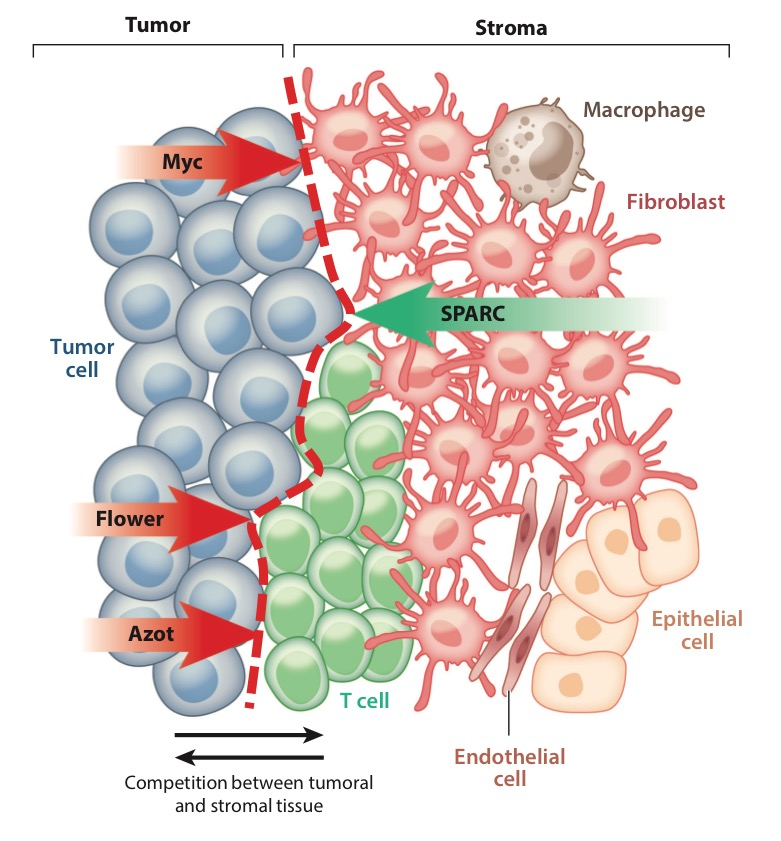
\includegraphics{images/04-1.jpg}

\begin{Shaded}
\begin{Highlighting}[]
\NormalTok{knitr}\OperatorTok{::}\NormalTok{opts_chunk}\OperatorTok{$}\KeywordTok{set}\NormalTok{(}\DataTypeTok{comment=}\OtherTok{NA}\NormalTok{, }\DataTypeTok{fig.width=}\DecValTok{1}\NormalTok{, }\DataTypeTok{fig.height=}\DecValTok{1}\NormalTok{)}
\end{Highlighting}
\end{Shaded}

Flower is a putative transmembrane protein that has three isoforms, two
are losers and one is a winner in Drosophila growing disc epithelium
(Rhiner Drosophila Dev Cell 2010). RNAi against the losers is sufficient
to make a cell a winner and vice versa for flower expressing cells in
Drosophila epithelium. When DMBA-TPA is used to promote papilloma
formation in mice, loser flower isotypes are expressed by surrounding
stromal cells, while winner flower isotypes are expressed by the
papilloma, suggesting that this mechanism is conserved from flies to
vertebrates (Petrova Dis Models Mech 2012).

Azot is an intracellular protein that integrates the information from
flower and SPARC both from the same cell and from surrounding cells and
decide if its cell should apoptose (Petrova Commun Integr Biol 2011). If
cells have low expression levels of loser flower isoform or high SPARC,
or surrounding cells have higher expression levels of loser flower, azot
is not transcribed and the cell will survive (Merino Cell 2015).

It might be possible that while tumor cells are growing and expanding,
they express fitness impacting genes like flower, Azot, and Myc, which
gives them a competitive advantage over surrounding stromal cells.

\section{Localization}\label{localization}

In the Drosophila gonad, both germline stem cells (GSCs) and somatic
stem cells (cyst progenitor cells, CPCs) share a niche created by
stromal cells that make up the hub and both share a requirement for
JAK-STAT signaling to maintain their stemness. This system provides an
understanding for how a single niche with multiple cell types is not
overrun by the one that cycles the most rapidly.

\begin{Shaded}
\begin{Highlighting}[]
\NormalTok{knitr}\OperatorTok{::}\KeywordTok{include_graphics}\NormalTok{(}\KeywordTok{rep}\NormalTok{(}\StringTok{"images/04-2.jpg"}\NormalTok{, }\DecValTok{1}\NormalTok{))}
\end{Highlighting}
\end{Shaded}

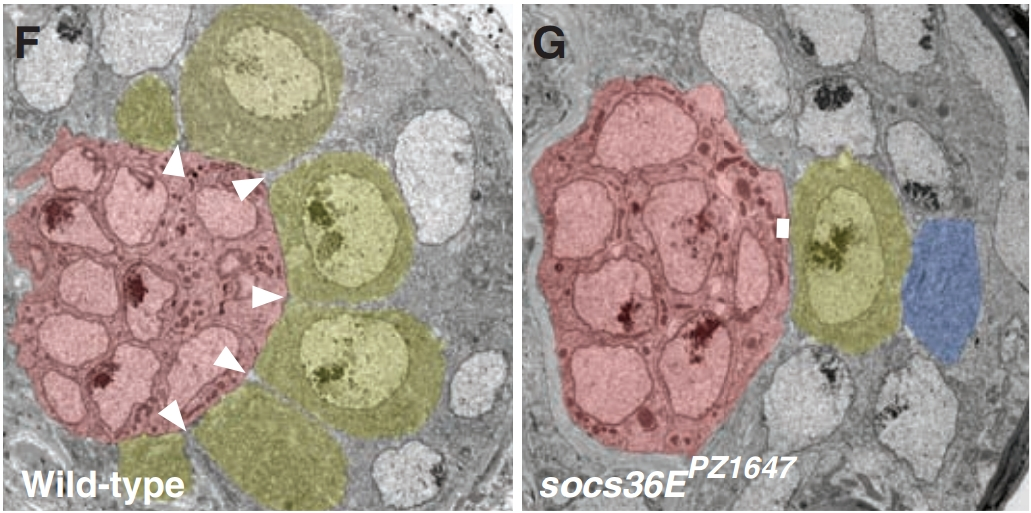
\includegraphics{images/04-2.jpg}

\begin{Shaded}
\begin{Highlighting}[]
\NormalTok{knitr}\OperatorTok{::}\NormalTok{opts_chunk}\OperatorTok{$}\KeywordTok{set}\NormalTok{(}\DataTypeTok{comment=}\OtherTok{NA}\NormalTok{, }\DataTypeTok{fig.width=}\DecValTok{1}\NormalTok{, }\DataTypeTok{fig.height=}\DecValTok{1}\NormalTok{)}
\end{Highlighting}
\end{Shaded}

In the Drosophila testis, suppressor of cytokine signaling (SOCS36E)
which is a JAK-STAT antagonist is expressed at high levels in the hub
and at low levels in the CPCs. The JAK-STAT signaling in part drives the
expression of position specific βPS-integrin which is used by both the
GSCs and the CPCs to bind and localize to the hub. The image to the
right shows in F how typically the GSCs (yellow) have a large surface
area integrin mediated connection with the hub, while CPCs (gray) only
make small integrin mediated connections. As shown in G, when SOCS36E is
inhibited in the CPCs, JAK-STAT signaling is downregulated resulting in
an upregulation of βPS-integrin which then allows the CPCs to bind more
readily to the hub. This increased surface area of association between
the hub and the CPCs allows the CPCs to outcompete the GSCs for binding
spots, and eventually results in loss of GPCs (Issigonis Science 2009).
Aberrant JAK-STAT signaling which includes loss of SOCS expression in
mammals(Bowman Oncogene 2000, Pontier J Cell Sci 2009, Leeman Expert
Opin Biol Ther 2006), and may play a role in stem cell misregulation
driven cancers (Reya Nature 2001).

Similar to mammals, germline stem cell transplants in Drosophila are
more efficient if the original GSCs are first depleted, supporting a
space-filling model of GSC-hub binding (Bhattacharya Eur J Imm 2008,
Oatley Ann Rev Cell Dev Bio 2008). Upon GSC loss, hub binding space is
freed, which drives dedifferentiation of somatic stem cells that then
fill the empty area adjacent to other GSCs (Sheng Cell Stem Cell 2009).

In the skin, collagen 17 (COL17A1), a component of the hemidesmosome,
fluctuates in response to genomic and oxidative stress induced
proteolysis. The stem cells that maintain high levels of COL17A1 are
able to maintain contact with the niche and symmetrically divide,
allowing them to outcompete neighbors that express low levels of COL17A1
as they will divide asymmetrically. With age it seems that all skin stem
cells begin to lose their COL17A1 expression and eventually start to
delaminate, and contributing to aging. Forced maintenance of COL17A1
however, seems to somewhat rescue skin aging \citep{liu2019stem}.

\section{Microenvironment}\label{microenvironment}

Lethal Giant Larvae (lgl) and scribble (scrib) are tumor suppressor
genes in Drosophila that play necessary roles in establishing cell
polarity and asymmetric cell divisions (Knoblich Cell 2008). Larvae that
are constitutively mutant for lgl develop diffuse, ultimately lethal
tumors, but clones of mutant cells surrounded by WT cells do not produce
tumors (Froldi BMC Biol 2010, Igaki Dev Cell 2009).

\begin{Shaded}
\begin{Highlighting}[]
\NormalTok{knitr}\OperatorTok{::}\NormalTok{opts_chunk}\OperatorTok{$}\KeywordTok{set}\NormalTok{(}\DataTypeTok{comment=}\OtherTok{NA}\NormalTok{, }\DataTypeTok{fig.width=}\DecValTok{1}\NormalTok{, }\DataTypeTok{fig.height=}\DecValTok{1}\NormalTok{)}
\NormalTok{knitr}\OperatorTok{::}\KeywordTok{include_graphics}\NormalTok{(}\KeywordTok{rep}\NormalTok{(}\StringTok{"images/04-3.jpg"}\NormalTok{, }\DecValTok{1}\NormalTok{))}
\end{Highlighting}
\end{Shaded}

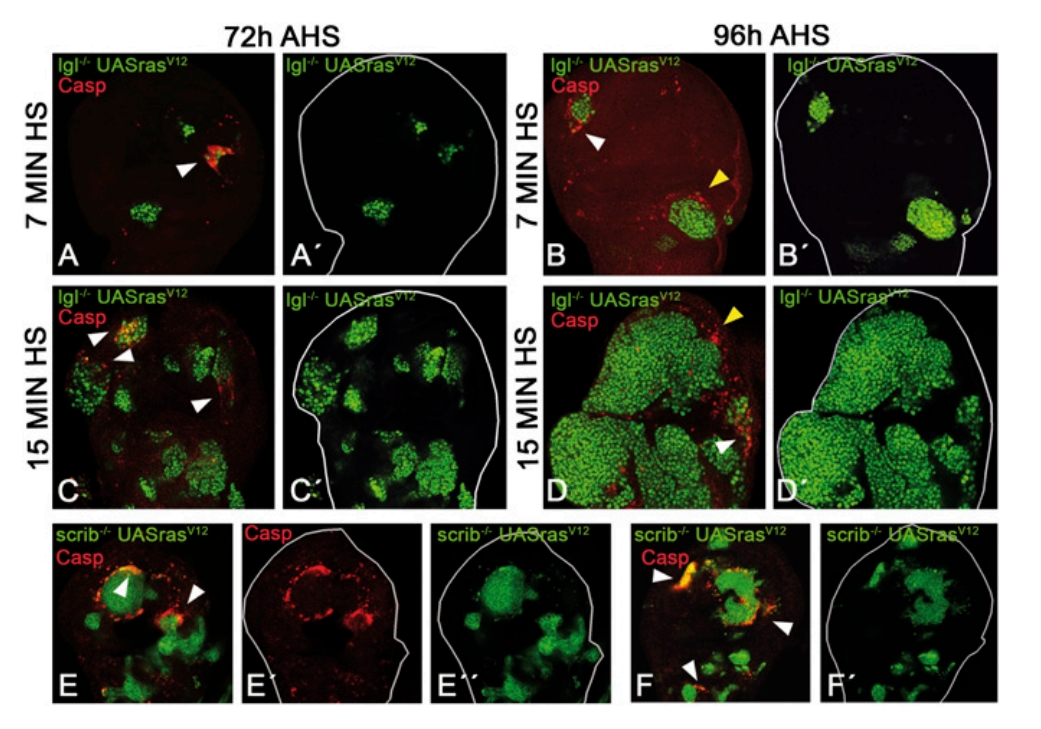
\includegraphics{images/04-3.jpg} It appears that scrib mutant cells
undergo JNK-driven apoptosis when surrounded by WT cells (Brumby EMBO
2003). This resembles minutes and Dpp cell competition (Moreno Nature
2002, Morata Dev Bio 1975). When lgl- cells are created using a heat
shock method in Drosophila in order to affect only a small percentage of
cells, the cells would still apoptose, and do so preferentially at the
border of clones indicating a short-range apoptosis inducing mechanism
originating from WT cells. Interestingly, when larvae were heat shocked
for different amounts of time, there was an exponential increase in
surviving non-apoptosing lgl cells (figure) (Menéndez et al. 2010). The
theory for why this occurs is that lgl- clones need to form a protective
niche to survive, and merging clones can facilitate this. This may solve
the riddle of how all oncogenic mutations could be present in a given
tissue and not give rise to a cancer, it may be that a critical mass of
oncogenically initiated cells is necessary before they can avoid WT cell
outcompetition.

\chapter{Bioinformatics}\label{bioinformatics}

\section{Genome stuff}\label{genome-stuff}

There are many instances of `NNN' repeats within the human genome,
because there are parts that are very challenging to sequence, including
telomere and centromere regions. Lowercase letters in the genome specify
things like repetitive sequences and introns. k-mers are fragments of
DNA in the genome that are of a length k, so for the string ATGCA, the
2-mers are AT, TG, GC, and CA, and the 3-mers are ATG, TGC, and GCA
k-mers can be useful for error correction because sequencing errors can
bias towards producing k-mers, but they can also be used in alignment or
in genome classification No free lunch theorem

\section{Software}\label{software}

Google has designed a new variant caller called DeepVariant that uses
deep neural networks to learn how best to call variants. This appears to
provide a significant improvement to variant calling accuracy (Poplin et
al., 2016).

A group put together well defined pipelines for common bioinfomatics
analysis like RNASeq into bioconductor that can be easily used and then
cited as a method of succinctly referring to the analysis process
(\url{http://www.nature.com/authors/policies/license.html}).

A group came up with a deep machine learning algorithm that can be used
to predict patient data and genomics patterns (Ching et al., 2017).

A group created a machine-learning algorithm for variant calling that
seems to significantly outperform many common variant calling software
like somatic sniper and mutect, though they do not compare against
freebayes. Might be worth taking a look at (Wood et al., 2018)

Selene is a deep learning python library designed using PyTorch that is
designed to ask questions using genomic and sequencing data
\citep{chen2019selene}. They also mention in their paper a number of
other deep learning python libraries specifically designed to analyze
genomics data, that may be worth checking out: DragoNN,
pysster\citep{budach2018pysster}, and Kipoi\citep{avsec2018kipoi}.

\chapter{Cancer}\label{cancer}

\section{Introduction}\label{introduction-3}

\subsection{Incidence Rates}\label{incidence-rates}

Time and age plays a major role in the occurrence of many cancers, where
typically the risk of suffering most cancers is about 2\% by the age of
40 in humans, while the risk increases to about 50\% by the age of 80
\citep{martincorena2015somatic}.

\begin{Shaded}
\begin{Highlighting}[]
\NormalTok{knitr}\OperatorTok{::}\KeywordTok{include_graphics}\NormalTok{(}\KeywordTok{rep}\NormalTok{(}\StringTok{"images/04-4.jpg"}\NormalTok{, }\DecValTok{1}\NormalTok{))}
\end{Highlighting}
\end{Shaded}

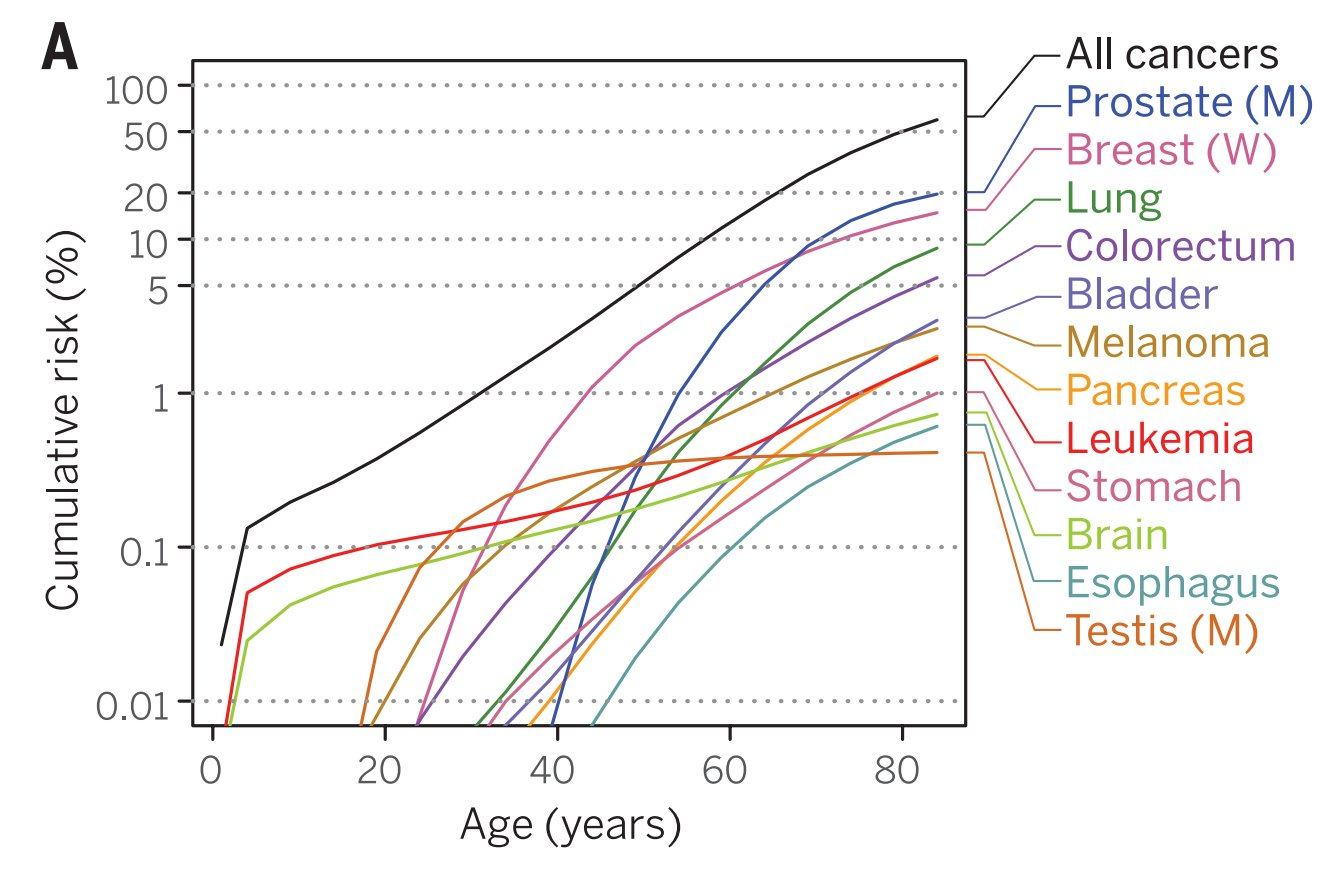
\includegraphics{images/04-4.jpg}

\bibliography{book.bib,packages.bib}


\end{document}
